\documentclass[11pt]{article}
\usepackage{latexsym}
\usepackage{amsmath}
\usepackage{amssymb}
\usepackage{amsthm}
\usepackage{epsfig}
\usepackage[tight]{subfigure}

\usepackage{amsmath}
\usepackage{hyperref}

\DeclareMathOperator*{\minimize}{min}
\DeclareMathOperator*{\maximize}{max}
\DeclareMathOperator*{\argmax}{arg\,max}
\DeclareMathOperator*{\argmin}{arg\,min}

\usepackage{algorithm}
 %on linux you may need to run sudo apt-get install texlive-full to install algorithm.sys
\usepackage{algorithmic}

\usepackage{verbatim}

\newcommand{\handout}[5]{
  \noindent
  \begin{center}
  \framebox{
    \vbox{
      \hbox to 5.78in { {#1} \hfill #2 }
      \vspace{4mm}
      \hbox to 5.78in { {\Large \hfill #5  \hfill} }
      \vspace{2mm}
      \hbox to 5.78in { {\em #3 \hfill #4} }
    }
  }
  \end{center}
  \vspace*{4mm}
}

\newcommand{\lecture}[5]{\handout{#1}{#2}{#3}{#4}{#5}}
\newcommand{\collision}[0]{\mathrm{collision}}
\newcommand{\nocollision}[0]{\overline{\collision}}

\newcommand*{\QED}{\hfill\ensuremath{\square}}

\newtheorem{theorem}{Theorem}
\newtheorem{corollary}[theorem]{Corollary}
\newtheorem{lemma}[theorem]{Lemma}
\newtheorem{observation}[theorem]{Observation}
\newtheorem{proposition}[theorem]{Proposition}
\newtheorem{definition}[theorem]{Definition}
\newtheorem{claim}[theorem]{Claim}
\newtheorem{fact}[theorem]{Fact}
\newtheorem{assumption}[theorem]{Assumption}
\newtheorem{note}[theorem]{Note}

% 1-inch margins, from fullpage.sty by H.Partl, Version 2, Dec. 15, 1988.
\topmargin 0pt
\advance \topmargin by -\headheight
\advance \topmargin by -\headsep
\textheight 8.9in
\oddsidemargin 0pt
\evensidemargin \oddsidemargin
\marginparwidth 0.5in
\textwidth 6.5in

\parindent 0in
\parskip 1.5ex
%\renewcommand{\baselinestretch}{1.25}

\begin{document}

\lecture{Statistical Techniques in Robotics (16-831, S22)}{Lecture \#09
  (Wednesday, Feb 16)}{Lecturer: Kris Kitani}{Scribes: Siqi Chai, Jiajie Xu (Group D)}{Online Gradient Descent }

\section{Review}
In the previous lecture, we discussed the relationship between Follow The Regularized Leader (FTRL) and Online Mirror Descent (OMD) algorithms. We showed that they are equivalent through reparametrizing dual parameters and the mirror function. We introduced the concept of duality and derived the regret bound for OMD. In this lecture, we will cover Gradient Descent and Stochastic Gradient Descent. In the online scenario, gradient descent is a type of OMD, and we will derive its regret bound.

%This section serves as a review of the previous lecture and any other context required to frame the content of the current lecture. 

%You may format the scribes in any way you like, aside from changing font style, size and page format. Please use subsections and paragraphs to increase the readability of your notes.

%Length requirement 1-2 pages.
        
\subsection{Mirror Function}
We recall that in order to show the equivalence between FTRL and OMD, we introduce the dual space. In FTRL, we optimize weight parameters \(w*\) in the primal space. In OMD, We optimize in the dual space and then map to primal space. Since the dual space is induced by the regularization term, \(\psi(w)\), the way we map from dual space back to primal space depends on the way we regularize. The mirror function, \(g(\theta)\) characterizes the mapping. In FTRL when we have a linear loss and convex regularization, we predict w as follow:
\[w^{(t+1)} = arg\min_{w}<w, z^{(1:t)}> + \psi(w)\]
we can convert it to a maximization problem by mapping to the dual space:
\[\theta^{(t+1)} := -z^{(1:t)}\]
The optimization problem now becomes:
\begin{equation*}
\begin{split}
    w^{(t+1)} &= arg\max_{w}<w, \theta^{(t+1)}> - \psi(w) \\
              &= g(\theta^{(t+1)})
\end{split}
\end{equation*}
This is how we convert a FTRL with linear loss and convex regularization into a OMD problem!


\subsection{OMD Regret Bound}

\definition{\normalfont\textbf{Convex Conjugate:}}
\normalfont
\[\psi^*(\theta) = max_{w}(<\theta, w>, - \psi(w))\]
The terms to be maximized is geometrically the difference between a function's value at w and the line with slope of the function at w. At the optimal w, the conjugate functional evaluates to the intercept of tangent of \(\psi(w)\). 

\normalfont\textbf{Fenchel-Young Inequality:}
\normalfont
\[\psi(\theta) \geq (<w, \theta> - \psi(w))\]
The proof for this comes directly from the definition of Convex Conjugate. When w takes whatever non-optimal value, the left hand side will evaluate to be grater than the right hand side.

\normalfont\textbf{Bregman Divergence:}
\normalfont
\[D_\psi(w||u) = \psi(w) - \psi(u) - \nabla\psi(u)^T(w - u)\]
The Bregman Divergence equation can be interpreted as a measurement of approximation error. The first two terms evaluates to the difference between function values at two distinct points. The last term is the first order approximation of the function. Note that \(\psi\) is a convex function.

\normalfont\textbf{OMD regret bound:}
\normalfont
\[R(u) = \sum_{t=1}^T w^{(t)}\cdot z^{(t)} - u \cdot z^{(t)}\]
Armed with the above tools, we're now ready to derive the regret bound for OMD defined above. By substituting in the dual parameter and applying Fenchel-Young Inequality we get:
\[\psi(u) - u \cdot \theta^{(T + 1)} \geq -\psi^*(\theta^{(T + 1)})\]
We show by telescoping technique that:
\[\psi(\theta^{(1)})  = -\psi(w ^ {(1)})\]
Finally by some algebra and Bregman Divergence, we have the upper bound of reget as:
\[R(u) \leq \psi(u) - \psi(w^{(1)}) + \sum_{t=1}^T D_{\psi^*} (-z^{1:t} || -z^{1:t-1})\]

\subsection{Main Take Away}
\begin{itemize}
    \item FTRL can be interpreted as OMD.
    \item The Mirror function depends on the regularization function, which then affects the regret bound.
    \item OMD is a generic algorithm to solve for online convex optimization.
\end{itemize}
\clearpage


\section{Summary}
\subsection{Gradient Descent: 3 interpretations}
\normalfont

\begin{algorithm}[H]
\caption{Gradient Descent}
\begin{algorithmic}[1]
\STATE $\textbf{w}^{(0)} \leftarrow {0}$ \hfill
\FOR{$t=1,\;\cdots,\;T$}
\STATE \textsc{COMPUTE} ($\nabla f(w^{(t-1)})$) \hfill
\STATE $w^{(t)} = w^{(t - 1)} - \eta \nabla f(w^{(t - 1)}) $  \hfill $\triangleright$ Weight update
\ENDFOR
\end{algorithmic}
\end{algorithm}

We are familiar with the Gradient Descent algorithm, but we may not know the reason behind it. It is intuitive to update the weights as in the pseudo-code: walking down the gradient, but we need some mathematical interpretations. There are three: 
\subsubsection*{Interpretation 1: Geometric}
\begin{figure}[H]
    \centering
    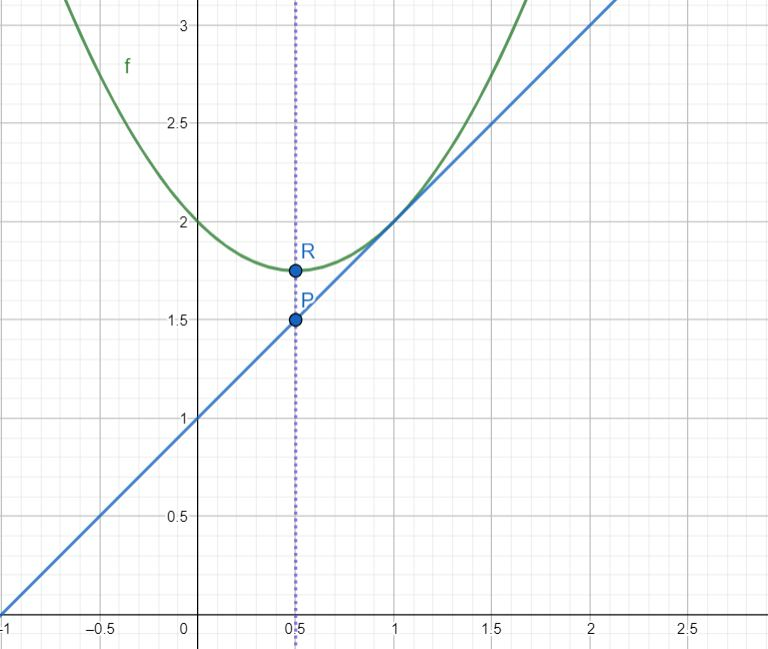
\includegraphics[width=0.3\textwidth]{pic/lo.jpg}
\end{figure}

From the geometric perspective, the optimal parameter always stay at the bottom of the 'hill', and that's why we should walk to the opposite direction of the gradient. Note that the gradient, which is the derivative of the objective function with respect to weight parameters, can be a scalar, a vector, or even  a matrix. It depends on what kind of objective function we have, and also the form of weight parameter.
\[\nabla f(w) = \{\frac{\delta f(w)}{\delta w_1}, \cdots, \frac{\delta f(w)}{\delta w_N}\}\]

\subsubsection*{Interpretation 2: Linear Approximation}
The geometric interpretation is a natural but not rigorous. Here, we give another more mathematical interpretation. We formulate the problem as a linear approximation problem. That is, we approximate the optimal weight, which gives the minimum loss, by first order Taylor approximation. 
\[f(u) \approx f(w) + <u-w, \nabla f(w)>\]
In the convex setting, we formulate the lower bound of \(f(u)\) as:
\[f(u) \geq f(w) + <u-w, \nabla f(w)>\]
We want to find the optimal w, that minimize the loss, thus we take the above inequality and minimize the right hand side. When we do so, however, we find that the result is negative infinity! Recall that the Taylor approximation only works for a small step size, thus we need to constraint w so that it is close to the previous value before update.
\[\min_w ||w - w^{(t)}||^2_2\]
With this constraint applied, the optimization function now have two parts:
\begin{itemize}
    \item minimize with linear approximation
    \item minimize the step size
\end{itemize}
Thus the final optimization formulation is:
\[w^{(t+1)} = arg min_w \eta \frac{1}{2} ||w - w^{(t)}||^2 + (f(w^{(t)}) + <w - w^{(t)}, \nabla f(w^{(t)})>)\]
Note that now we have a linear loss and a quadratic regularization!

\subsubsection*{Interpretation 3: Isometric Quadratic Approximation}
In the previous section, we applied the first order Taylor approximation. We can take it further by using the second order Taylor approximation. That is, we approximate the gradient with second order derivative, and reduce the approximation error. The new optimization looks like:
\[f(u) \approx f(w) + (u-w)^T\nabla f(w) + \frac{1}{2} (u-w)^T \nabla^2 f(w)(u-w)\]
Again, in a convex condition, the right hand side is the lower bound of approximation:
\[f(u) \geq f(w) + (u-w)^T\nabla f(w) + \frac{1}{2} (u-w)^T \nabla^2 f(w)(u-w)\]
Generally speaking, computing the second order derivative with respect to w is expensive. Assume w is a n-d vector:
\[O(hessian) = O(n^2)\]
\[O(derivative) = O(n)\]
This computation takes quadratic time and we need to reduce it! Here we simplify the hessian matrix to a identity matrix:
\[f(u) \geq f(w) + (u-w)^T\nabla f(w) + \frac{1}{2\eta} (u-w)^T I(u-w)\]
We will be using this formulation later in Support Vector Machine (SVM).

\subsubsection*{Solving the optimization}
We proceed to solve the optimization problem defined in prospective 2. 
\[w^{(t+1)} = arg min_w \eta \frac{1}{2} ||w - w^{(t)}||^2 + (f(w^{(t)}) + <w - w^{(t)}, \nabla f(w^{(t)})>)\]
Our goal is to find a better weight, \(w^{(t+1)}\), that will reduce the loss function. In order to solve it, we take the derivative and set the derivative to 0 (refer to \hyperref[sec:App Solving the optimization]{Appendix 3.1} for details):
\begin{align*}
    w &= w^{(t)} - \eta \nabla f(w^{(t)})
\end{align*}
Now we have it! The above weight update function was seen in the Weighted Majority Algorithm (WMA), the Online Perceptron Algorithm, as well as the Follow The Regularized Leader algorithm (FTRL).




\subsection{Stochastic Gradient Descent}
\normalfont
\begin{algorithm}[H]
\caption{Stochastic Gradient Descent}
\begin{algorithmic}[1]
\STATE $\textbf{w}^{(1)} \leftarrow {0}$ \hfill
\STATE $\eta > 0$ \hfill
\FOR{$t=1,\;\cdots,\;T$} 
\STATE \textsc{SAMPLE} ($z \sim D $) \hfill $\triangleright$ Sample from data distribution
\STATE \textsc{COMPUTE} ($\nabla f_z(w^{(t-1)})$) \hfill $\triangleright$ Fast to compute
\STATE $w^{(t)} = w^{(t - 1)} - \eta \nabla f_z(w^{(t - 1)}) $  \hfill $\triangleright$ Weight update
\ENDFOR
\end{algorithmic}
\end{algorithm}
Each iteration of gradient descent update can be computationally expensive given a large dataset. In fact, as long as we can eventually arrive at the bottom of the 'hill', we do not need to always take the globally optimal path. That is, we can take gradient descent steps according to a small batch of data as long as the expected direction equal the gradient direction. We will save a lot computation if we only calculate the gradient on a mini-batch. Still, the convergence bound of SGD is smiliar to that of gradient descent.
\begin{figure}[H]
    \centering
    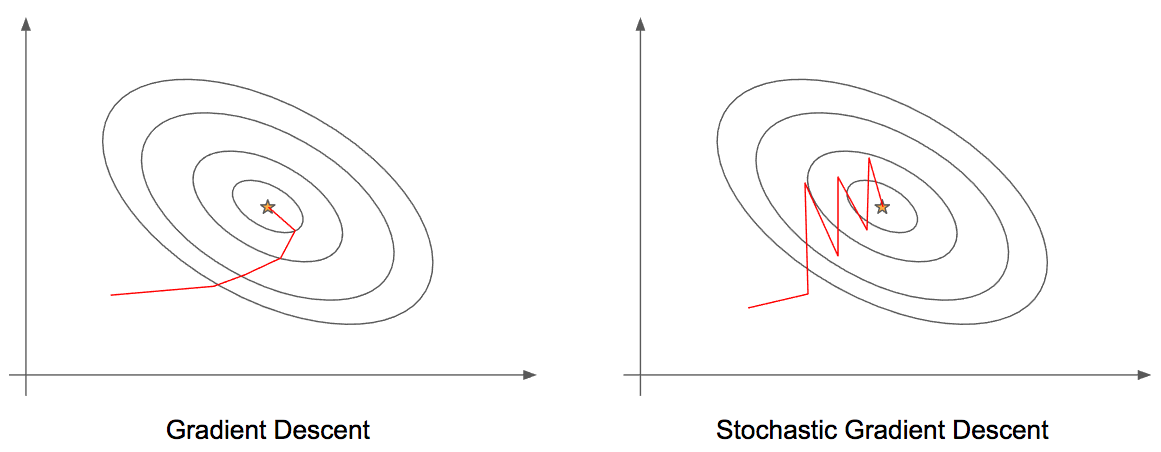
\includegraphics[width=0.7\textwidth]{pic/GD-v-SGD.png}
\end{figure}

\theorem{(SGD/OGD is special case OMD)}
\begin{algorithm}[H]
\caption{Online Sub-Gradient Descent}
\begin{algorithmic}[1]
\FOR{$t=1,\;\cdots,\;T$} 
\STATE $\theta^{(t+1)} = \theta^{(t)} - z^{(t)}, z^{(t)} \in \delta f^{(t)}(w^{(t)})  $ \hfill $\triangleright$ Dual Parameter update with magnitude assumption
\STATE $w^{(t + 1)} = \eta \theta^{(t + 1)}$  \hfill $\triangleright$ Mirror projection
\ENDFOR
\end{algorithmic}
\end{algorithm}

\begin{algorithm}[H]
\caption{Online Proj Sub-Gradient Descent}
\begin{algorithmic}[1]
\FOR{$t=1,\;\cdots,\;T$} 
\STATE $\theta^{(t+1)} = \theta^{(t)} - z^{(t)}, z^{(t)} \in \delta f^{(t)}(w^{(t)})  $ \hfill $\triangleright$ Dual Parameter update
\STATE $w^{(t + 1)} = \Pi_{(\theta \rightarrow s)} \eta \theta^{(t + 1)}$  \hfill $\triangleright$ Mirror projection with explicit feasibility condition
\ENDFOR
\end{algorithmic}
\end{algorithm}

\proof{Define a OMD with linear loss can quadratic regularization, show the mirror function is same as OGD:\\
Quadratic Regularization:
\[\psi(w) = \frac{1}{2\eta} ||w||^2_2\]
Linear Loss:
\[f(w) = <w, \theta>\]
Then we have a prediction rule:
\begin{equation}
    \begin{split}
    w^{(1 + t)} &= arg \min_w <w, -\theta^{(1 + t)}> + \frac{1}{2\eta} ||w||^2_2 \\
    &= arg \min_w <w, -\theta^{(1 + t)}> + \frac{1}{2\eta} \sum_n w^2_n\\
\end{split}
\end{equation}
We define the right hand side as a loss function, and minimize it by taking the derivative:
\[L = <w, -\theta^{(1 + t)}> + \frac{1}{2\eta} \sum_n w^2_n\]
\[\frac{\delta L}{\delta w_n} = -\theta_n + \frac{1}{2\eta} 2 w_n = 0\]
\[w_n = \eta \theta_n\]
Recall that the OMD mirror function is:
\[g(\theta) = \eta \theta\] \QED}\\
These are exactly the same! Thus, OGD is a special case of OMD. Note that we gave two versions of the algorithm: Online Sub-Gradient Descent (Alg.3) and Online Proj Sub-Gradient Descent. The difference between the two is that in Online Sub-Gradient Descent we do not need to actually project from dual space to primal space. That is, on line 3 of the pseudo code, we update w by multiplied \(\theta\). The simplicity comes from the assumption that the dual space gradient has a constrained magnitude. In the Online Proj Sub-Gradient Descent, we need to project from dual space to primal space with the funtion \(\Pi_{(\theta \rightarrow s)}\). For example, we can use the eucilidian projection:
\[\Pi_{(\theta \rightarrow s)} (x) = arg\min_y ||x-y||^2\]

\subsection{OGD Regret Bound}
\normalfont

\theorem{(Regret Bound of Online Gradient Descent) with assumed maximum magnitude of primal parameter D and assumed maximum magnitude of dual parameter sub-gradient G}
\[R_{OGD} \leq DG\sqrt{T}\]
where
\[\psi(w) = \frac{1}{2\eta} ||w||^2_2\]
\[D = max||u||^2, u \in S\]
\[G = max||z||^2, u \in \delta f(w)\]

\lemma{Under L2 norm, the convex conjugate function is in the same form as the regularizing function:}
\[\psi(w) = \frac{1}{2} ||w||^2_2\]
\[\psi^*(\theta) = \frac{1}{2} ||\theta||^2_2\]
\proof{
\begin{equation}
    \begin{split}
        \psi^*(\theta) &= \max_w (<\theta, w > - \psi(w)) \\
        &= -\min_w(\psi(w) - <\theta, w >)
    \end{split}
\end{equation}
\begin{equation}
    \begin{split}
        -\psi^*(\theta) &= \min_w(\psi(w) - <\theta, w >)\\
        &= \min_w(\frac{1}{2} ||w||^2_2 - <\theta, w >)
    \end{split}
\end{equation}
To minimize, we take the derivative and set it to 0
\begin{equation}
    \begin{split}
        \frac{\delta}{\delta w}\{\frac{1}{2} ||w||^2_2 - <\theta, w >\} &= 0 \\
        w - \theta &= 0\\
        w &= \theta
    \end{split}
\end{equation}
Now we plug in w to the convex conjugate function (refer to \hyperref[sec:Solving the convex conjugate]{Appendix 3.2}):
\[\psi^*(\theta) = \frac{1}{2} ||\theta||^2_2\] \QED}

\proof{(Regret bound of OGD) As shown previously, OGD is a special case of OMD, thus we start by the regret formulation for OMD:
\[R(u) \leq \psi(u) - \psi(w^{(1)}) + \sum_{t=1}^T D_{\psi^*} (\theta^{(t + 1)} || \theta^{(t)})\]
By Bregman Divergence, we can substitute the last term:
\[R(u) \leq \psi(u) - \psi(w^{(1)}) + \sum_{t=1}^T \psi^*(\theta^{(t + 1)}) - \psi^*(\theta^{(t)}) - \nabla \psi^*(\theta^{(t)})(\theta^{(t + 1)} - \theta^{(t)})\]
We plug in the defined regularizing function and derived convex conjugate function from Lemma 4 (\hyperref[sec:Algebra1]{Algebra in Appendix 3.3}):
\begin{equation}
    \begin{split}
        R(u) &\leq \frac{1}{2\eta} ||u||^2_2 - \frac{1}{2\eta} ||w^{(1)}||^2_2 + \sum_{t=1}^T \frac{1}{2\eta} ||\theta^{(t+1)}||^2_2 - \frac{1}{2\eta} ||\theta^{(t)}||^2_2 - \nabla \frac{1}{2\eta} ||\theta^{(t)}||^2_2(\theta^{(t + 1)} - \theta^{(t)}) \\
    \end{split}
\end{equation}
By update rule of \(\theta\):
\[\theta^{(t + 1)} = \theta^{(t)} - \eta z^{(t)}\]
We have (\hyperref[sec:Algebra2]{Algebra in Appendix 3.4}):
\begin{equation}
    \begin{split}
        R(u) &\leq \frac{1}{2\eta} ||u||^2_2 + \sum_{t=1}^T \frac{\eta}{2}||z^{(t)}||^2_2\\
    \end{split}
\end{equation}
Recall the definition of D and G:
\[D = max||u||^2, u \in S\]
\[G = max||z||^2, u \in \delta f(w)\]
Plugging in we have:
\begin{equation}
    \begin{split}
        R(u) &\leq \frac{1}{2\eta} ||u||^2_2 + \sum_{t=1}^T \frac{\eta}{2}||z^{(t)}||^2_2\\
        &\leq \frac{D^2}{2\eta} + \frac{\eta}{2}TG^2\\
    \end{split}
\end{equation}
We need to figure out the optimal step size \(\eta\). Again, we take the derivative and set it to 0 (\hyperref[sec:Algebra3]{Appendix 3.5}):
\begin{align*}
    \frac{\delta}{\delta \eta} \frac{D^2}{2\eta} + \frac{\eta}{2}TG^2 &= 0\\
    \eta &= \frac{D}{G\sqrt{T}}
\end{align*}
Now we plug the optimal \(\eta\) back and solve for the regret bound:
\begin{equation}
    \begin{split}
        R(u) &= DG\sqrt{T}
    \end{split}
\end{equation} \QED
}\\
We've completed the proof of OGD regret bound.


\subsection{Online Normalized Exponentiated Gradient Descent}
Online normalized exponentiated gradient descent (ONEGD) is an specific type of online mirror descent, with linear loss and entropic regularization. In practice, it may give the advantage of normalzing gradient make it more stable. Algorithm pseudocode:

\begin{algorithm}[H]
\caption{Online Norm-Exponentiated-Gradient($\eta$)}
\label{algo:onegd}
\begin{algorithmic}[1]
\FOR{$t=1,\;\cdots,\;T$}
\STATE $\boldsymbol{\theta}^{(t+1)} = \boldsymbol{\theta}^{(t)} - \eta \boldsymbol{z}^{(t)}, \quad \boldsymbol{z}^{(t)} \in \partial f^{(t)}(\boldsymbol{w}^{(t)})$ \hfill $\triangleright$ Dual parameter update
\STATE $\boldsymbol{w}^{(t+1)} \propto \boldsymbol{w}^{(t)} \exp{(\eta \boldsymbol{z}^{(t)})}$ \hfill $\triangleright$ Mirror projection
\ENDFOR
\end{algorithmic}
\end{algorithm}

\subsubsection{Loss and regularization setup}
Define regularization term as negative entropy with K-simplex constraint:
\[ \psi(\boldsymbol{w}) = \sum_{k=1}^{K} w_k \log w_k \quad \boldsymbol{w} \in \mathbb{S}^K \]
% Simplex is used to represent a probability distribution \\
This constraint is used when solution space is a probability simplex. The simplex constraint means each dimension of $\boldsymbol{w}$ sums up to 1: $\sum_k w_k = 1$. In the example below where $K=3$, solution space of $\boldsymbol{w}$ is inside the triangle.
\begin{figure}[H]
    \centering
    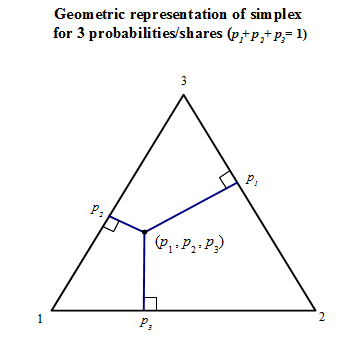
\includegraphics[width=0.5\textwidth]{pic/probability simplex.png} \cite{simplex_img}
\end{figure}

Define loss function as linear:
\[ f(\boldsymbol{w}) = \langle \boldsymbol{w}, \boldsymbol{\theta} \rangle \]

Recall, the parameter update equation for online mirror descent, substitute regularization term:
\begin{align}
    \boldsymbol{w}^{(t+1)} = & \argmin_{\boldsymbol{w}} \langle \boldsymbol{w}, -\boldsymbol{\theta}^{(t+1)} \rangle + \psi (\boldsymbol{w})\nonumber \\
    = & \argmin_{\boldsymbol{w} \in \mathbb{S}^K} \langle \boldsymbol{w}, -\boldsymbol{\theta}^{(t+1)} \rangle + \sum_{k=1}^{K} w_k \log w_k \nonumber
\end{align}
Add simplex constraint to the parameter update as Lagrange multiplier:
\[ \boldsymbol{w}^{(t+1)} = \argmin_{\boldsymbol{w} \in \mathbb{S}^K} \langle \boldsymbol{w}, -\boldsymbol{\theta}^{(t+1)} \rangle + \sum_{k=1}^{K} w_k \log w_k + \lambda \left( 1- \sum_k w_k \right) \]
When adding simplex constraint to objective function, we can rewrite it as Lagrangian expression:
\[ \mathcal{L} = \langle \boldsymbol{w}, -\boldsymbol{\theta}^{(t+1)} \rangle + \frac{1}{\eta}\sum_{k=1}^{K} w_k \log w_k + \lambda \left( 1- \sum_k w_k \right) \]
$\frac{1}{\eta}$ here is to balance the weight between loss and regularization term. \\

\subsubsection{Minima of Lagrangian}
To solve the minima of $ \mathcal{L} $, take its gradient to $\boldsymbol{w}$ and set it equal to 0. First, calculate partial derivative with respect to each element of $\boldsymbol{w}$:
\[ \frac{\partial \mathcal{L}}{\partial w_n} = -\theta_n + \frac{1}{\eta} (1 + \log w_n) - \lambda = 0 \]
Solve for $w_n$:
\[ w_n = \frac{\exp (\eta \theta_n)}{\exp (1 - \eta\lambda)} \]

Dual parameter update of OMD:
\[ \boldsymbol{\theta}^{(t+1)} = \boldsymbol{\theta}^{(t)} - \eta\boldsymbol{z}^{(t)}, \quad \boldsymbol{z}^{(t)} \in \partial f^{(t)}(\boldsymbol{w}^{(t)}) \]
Recall, definition of mirror/linking function: $\boldsymbol{w} = g(\boldsymbol{\theta})$, combine the partial derivatives. Mirror function enforces geometry of problem, we have:  %(TODO: How to solve $\lambda$?)
\[ g(\boldsymbol{\theta}) = \frac{\exp (\eta \boldsymbol\theta)}{\sum_k\exp(\eta\theta_k)} \]

To get the update equation for primal parameter $\boldsymbol{w}$ in incremental form, we start from this mirror function.
The key here is to substitute incremental form of dual parameter $\boldsymbol{\theta}$, and multiply a temporary term with the same sum of exponential on numerator and denominator:
\begin{align}
w_n^{(t+1)} = & \frac{\exp (\eta \theta_n^{(t+1)})}{\sum_k\exp(\eta\theta_k)} \nonumber \\
= & \frac{\exp \left(\eta (\theta_n^{(t)} - z_n^{(t)})\right) }{\sum_{k} \exp \left( \eta (\theta_k^{(t)} - z_k^{(t)}) \right)} \nonumber \hfill && \triangleright \text{incremental form of } \theta \\
= & \exp (\eta {\theta}_n^{(t)}) \frac{\exp (-\eta {z}_n^{(t)})}{\sum_k \exp (\eta {\theta}_k^{(t)}) \exp (-\eta {z}_k^{(t)})} \cdot \frac{\sum_j \exp (\eta {\theta}_j^{(t)})}{\sum_j \exp (\eta {\theta}_j^{(t)})} \nonumber && \triangleright \text{temporary term} \\
= & \frac{\exp (\eta {\theta}_n^{(t)})}{\sum_j \exp (\eta {\theta}_j^{(t)})} \cdot \exp (-\eta {z}_n^{(t)}) \cdot \frac{\sum_j \exp (\eta {\theta}_j^{(t)})}{\sum_k \exp (\eta {\theta}_k^{(t)}) \exp (-\eta {z}_k^{(t)})} \nonumber && \triangleright \text{rearrange terms} \\
= & \frac{{w}_n^{(t)} \exp (-\eta z_n^{(t)})}{\sum_k {w}_k^{(t)} \exp (- \eta z_k^{(t)})} \nonumber && \triangleright \text{substitute with def of }w
\end{align}

Therefore, we can get: $ w_n^{(t+1)} \propto w_n^{(t)} \exp (-\eta z_n^{(t)})$ \\
This is the same exponential update rule as weighted majority algorithm. % TODO: why?

\subsubsection{Connection to Hedge algorithm}
The hedge algorithm is similar to the weighted majority algorithm, with different exponential update rule. Hedge is an unnormalized exponentiated gradient descent algorithm.
\begin{algorithm}[H]
\caption{Hedge Algorithm($\beta$)}
\begin{algorithmic}[1]
\STATE $\boldsymbol{w}^{(1)} \leftarrow \{w_n^{(1)}=1\}_{n=1}^N$
\FOR{$t=1,\;\cdots,\;T$}
\STATE \textsc{Receive} ($\boldsymbol{x}^{(t)}\in\{-1, 1\}$)
\STATE $i\sim$ \textsc{Multinomial}($\boldsymbol{w}^{(t)}/\Phi^{(t)}$), $\Phi^{(t)}=\sum_{n=1}^Nw_n^{(t)}$
\STATE $\hat{y}^{(t)}=h_i(\boldsymbol{x}^{(t)})$ \hfill $\triangleright$ Expect 0-1 loss, linear
\STATE \textsc{Receive} ($y^{(t)}\in\{-1, 1\}$)
\STATE $w_n^{(t+1)} =  w_n^{(t)}e^{-\beta\cdot\boldsymbol{1}[y^{(t)}\neq h_n(\boldsymbol{x}^{(t)})]}, \forall n$ \hfill $\triangleright$ Exponential weight update
\ENDFOR
\end{algorithmic}
\end{algorithm}


%\section*{References}
%Include your references here. Please cite any resources you found useful.	
%Populate the refs.bib file or list your references manually. Be consistent in formatting!
{
\bibliography{refs}
\bibliographystyle{abbrv}
}

\section{Appendix}
%This section provides any relevant background material that was not covered in the lectures, but was found to be useful for understanding the material. 
%For example, derivations, theory underlying techniques employed, etc. 

%Additionally, this section can summarizes applications or extensions of these techniques found in the literature. 
\subsection{Solving the optimization}
\label{sec:App Solving the optimization}
\begin{align*}
    \frac{\delta}{\delta w} \{\eta \frac{1}{2} ||w - w^{(t)}||^2 + (f(w^{(t)}) + <w - w^{(t)}, \nabla f(w^{(t)})>) \} &= 0 \\
    \frac{1}{2} (2w + 0 -2w^{(t)}) + \eta (0 + \nabla f(w^{(t)}) - 0) &= 0 \\
    w - w^{(t)} + \eta \nabla f(w^{(t)}) &= 0 \\
    w &= w^{(t)} - \eta \nabla f(w^{(t)}) \\
\end{align*}

\subsection{Solving the convex conjugate}
\label{sec:Solving the convex conjugate}
\begin{equation}
    \begin{split}
        -\psi^*(\theta) &= \frac{1}{2} ||w||^2_2 - <\theta, w > \\
        &= \frac{1}{2} ||\theta||^2_2 - <\theta, \theta> \\
        &= -\frac{1}{2} ||\theta||^2_2
    \end{split}
\end{equation}

\subsection{Algebra used in regret bound proof}
\label{sec:Algebra1}
\begin{equation}
    \begin{split}
        R(u) &\leq \frac{1}{2\eta} ||u||^2_2 - \frac{1}{2\eta} ||w^{(1)}||^2_2 + \sum_{t=1}^T \frac{1}{2\eta} ||\theta^{(t+1)}||^2_2 - \frac{1}{2\eta} ||\theta^{(t)}||^2_2 - \nabla \frac{1}{2\eta} ||\theta^{(t)}||^2_2(\theta^{(t + 1)} - \theta^{(t)}) \\
        &= \frac{1}{2\eta} ||u||^2_2 - \frac{1}{2\eta} ||w^{(1)}||^2_2 + \sum_{t=1}^T \frac{1}{2\eta} ||\theta^{(t+1)}||^2_2 - \frac{1}{2\eta} ||\theta^{(t)}||^2_2 - \frac{1}{\eta} \theta^{(t)} (\theta^{(t + 1)} - \theta^{(t)}) \\
        &= \frac{1}{2\eta} ||u||^2_2 - \frac{1}{2\eta} ||w^{(1)}||^2_2 + \sum_{t=1}^T ||\theta^{(t+1)} - \theta^{(t)}||^2_2
    \end{split}
\end{equation}

\subsection{More Algebra used in regret bound proof}
\label{sec:Algebra2}
\begin{equation}
    \begin{split}
        R(u) &\leq \frac{1}{2\eta} ||u||^2_2 - \frac{1}{2\eta} ||w^{(1)}||^2_2 + \sum_{t=1}^T ||\theta^{(t)} - \eta z^{(t)} - \theta^{(t)}||^2_2\\
        &= \frac{1}{2\eta} ||u||^2_2 - \frac{1}{2\eta} ||w^{(1)}||^2_2 + \sum_{t=1}^T ||- \eta z^{(t)}||^2_2\\
        &\leq \frac{1}{2\eta} ||u||^2_2 + \sum_{t=1}^T \frac{\eta}{2}||z^{(t)}||^2_2
    \end{split}
\end{equation}

\subsection{Solving for optimal \(\eta\)}
\label{sec:Algebra3}
\begin{align*}
    \frac{\delta}{\delta \eta} \frac{D^2}{2\eta} + \frac{\eta}{2}TG^2 &= 0\\
    \frac{-D^2}{2\eta^2} + \frac{TG^2}{2} &= 0\\
    \frac{-D^2}{2} + \frac{\eta^2TG^2}{2} &= 0\\
    \eta^2 &= \frac{D^2}{TG^2} \\
    \eta &= \frac{D}{G\sqrt{T}}
\end{align*}

\subsection{Lagrange multiplier}
Lagrange multipliers is a strategy for finding the local maxima and minima of a function ($f(x)$) subject to equality constraints ($g(x)$). \cite{wiki:lagrange} It can convert this hard constraint into a term in the function, such that the derivative test of an unconstrained problem can still be applied. The general equation of this method is:
\[ \mathcal{L}(x,\lambda) = f(x) - \lambda g(x) \]

Here we show a simple example involving single constraint to help understand this method:

We want to find minima of $f(x,y) = x^2y$ with constraint $ x^2+y^2 = 1 $\\
Then, the constraint term can be represented as:
\[ g(x,y) = x^2+y^2-1 \]
And the Lagrangian expression is:
\[ \mathcal{L}(x,y,\lambda) = f(x,y) - \lambda g(x,y) = x^y + \lambda (x^2+y^2-1) \]
Set the partial derivative of this equation to 0 and get an equation set:
\begin{equation}
\begin{cases}
  2xy + 2\lambda x = 0 \\
  x^2 + 2xy = 0 \\
  x^2+y^2-1 = 0  \nonumber
\end{cases}       
\end{equation}
The minima we're looking for is one of the solutions of this equation set.

\subsection{Simplex}
In geometry, a simplex is a generalization of the notion of a triangle or tetrahedron to arbitrary dimensions. The simplex is so-named because it represents the simplest possible polytope in any given space. \cite{wiki:simplex} \\
A k-simplex is a k-dimensional polytope which is the convex hull of its k + 1 vertices (0-faces). Specifically:
\begin{itemize}
    \item a 0-simplex is a point
    \item a 1-simplex is a line segment
    \item a 2-simplex is a triangle
    \item a 3-simplex is a tetrahedron
\end{itemize}
\begin{figure}[H]
    \centering
    
\includegraphics[width=0.5\textwidth]{pic/Simplexes visual.jpg} \cite{wiki:simplex}
\end{figure}

However, when we talk about probability simplex, it is a mathematical space where each point represents a probability distribution between a finite number of mutually exclusive events. \cite{prob_simplex}. "Mutually exclusive" means a point on a probability simplex can be represented by K non-negative numbers that add up to 1. Geometrically, it is the $\mathbf{k-1}$ \textbf{dimensional} simplex whose vertices are the k standard unit vectors, because the requirement that the numbers sum to 1 reduces the dimensionality by 1.

\end{document} % Done!
